\documentclass{standalone}
\usepackage{tikz}
\usetikzlibrary{patterns, positioning}
\usepackage[sfdefault]{ClearSans} %% option 'sfdefault' activates Clear Sans as the default text font
\usepackage[T1]{fontenc}

\begin{document}
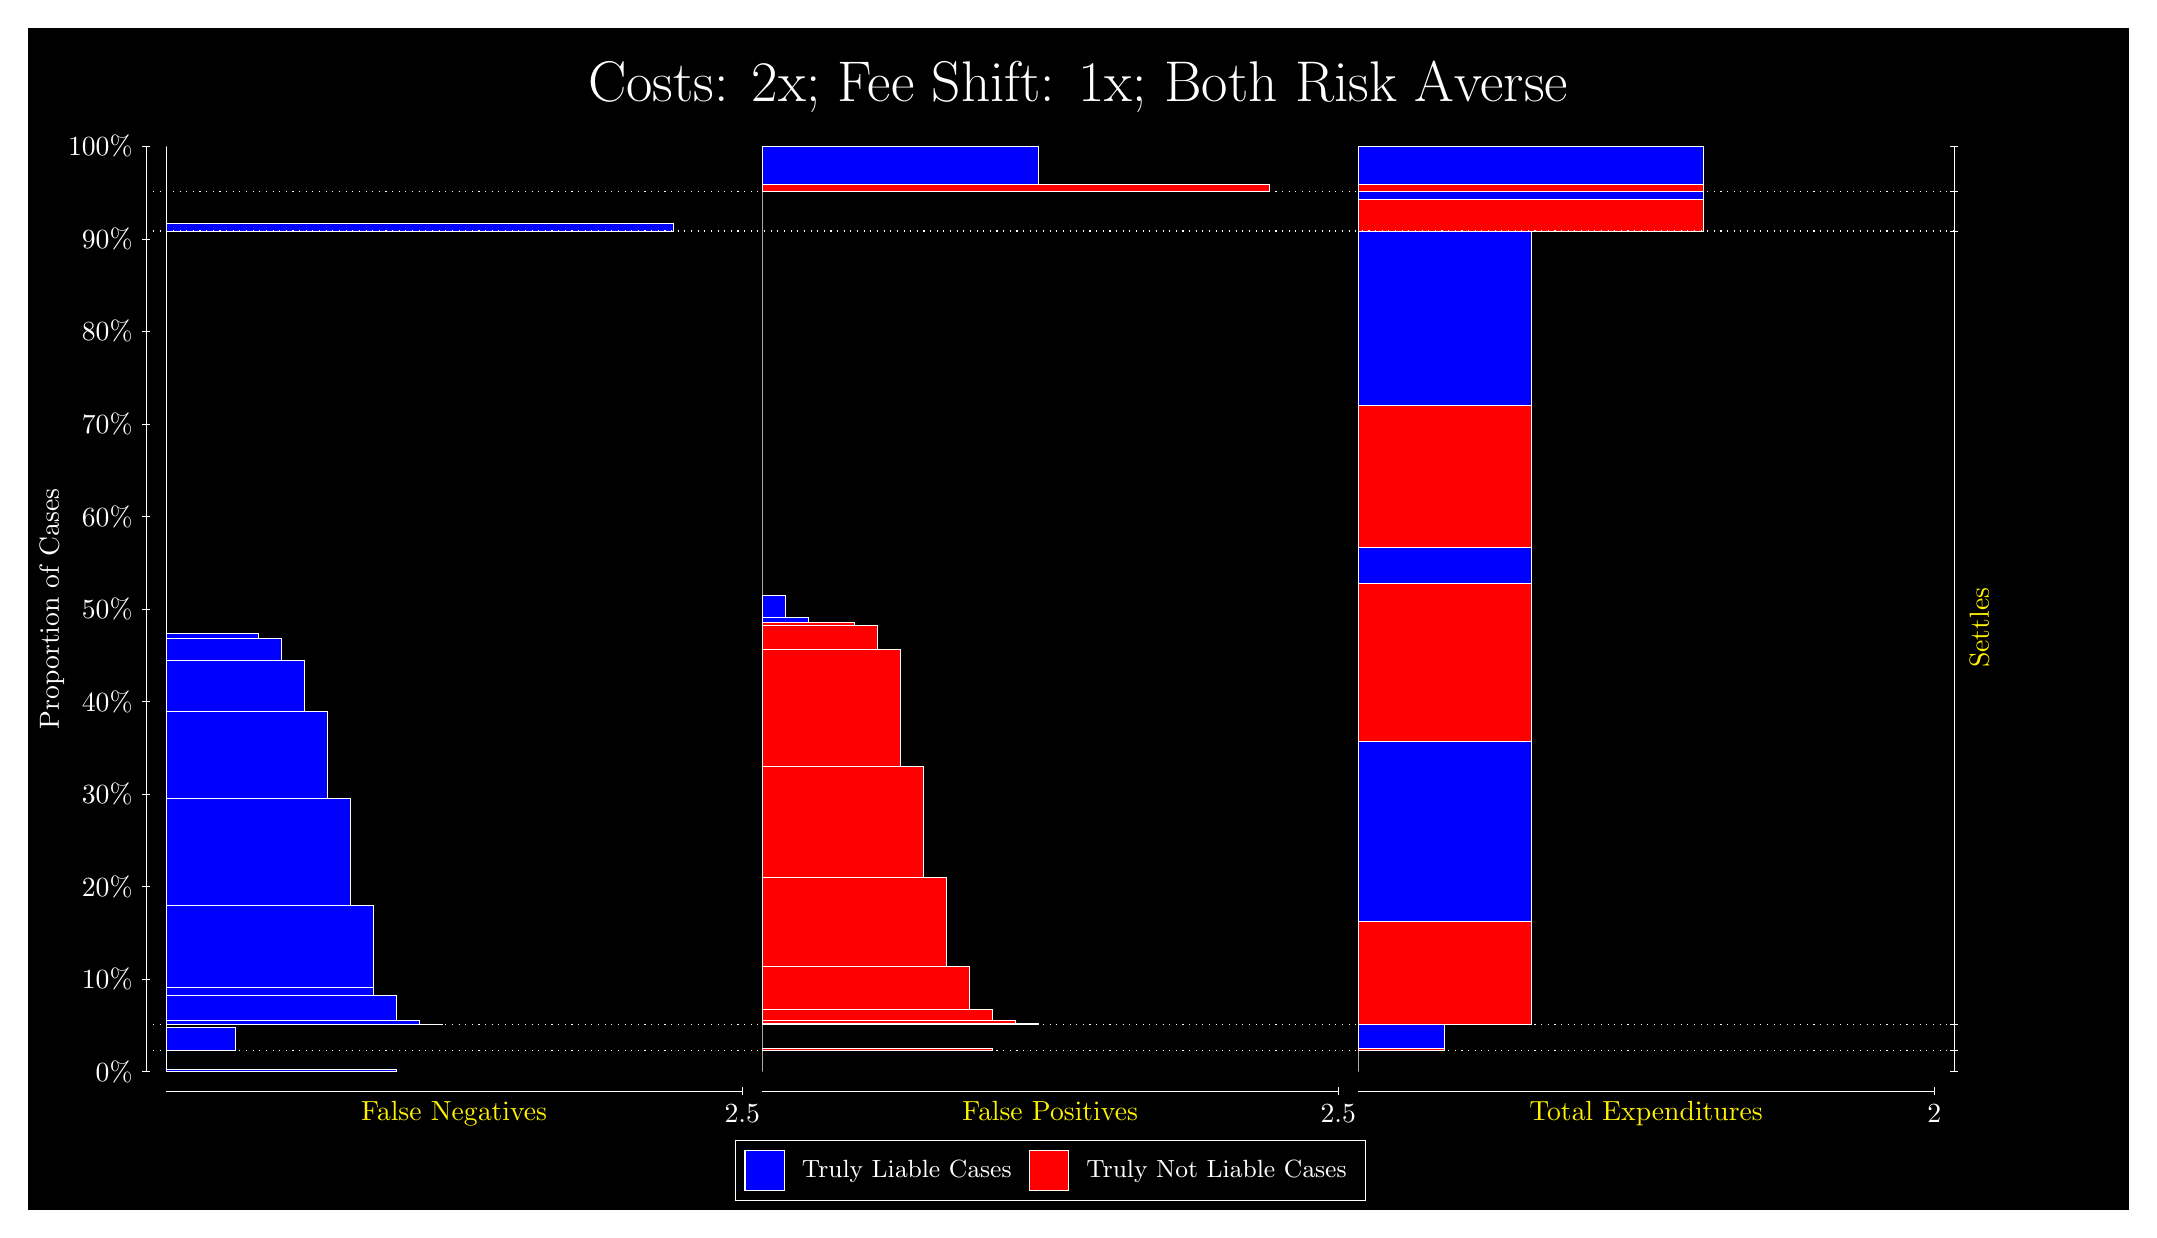
\begin{tikzpicture}
\draw[fill=black] (0,0) rectangle (26.667,15);
\draw[text=white] (0,13.5) rectangle (26.667,15) node[midway] {\huge Costs: 2x; Fee Shift: 1x; Both Risk Averse};
\draw[white, very thin] (1.5,1.75) -- (1.5,13.5);
\node[rotate=90, text=white, anchor=center] at (0.3, 7.625) {Proportion of Cases};
\draw[white, very thin] (1.45,1.75) -- (1.55,1.75);
\node[text=white, anchor=east] at (1.45, 1.75) {0\%};
\draw[white, very thin] (1.45,2.925) -- (1.55,2.925);
\node[text=white, anchor=east] at (1.45, 2.925) {10\%};
\draw[white, very thin] (1.45,4.1) -- (1.55,4.1);
\node[text=white, anchor=east] at (1.45, 4.1) {20\%};
\draw[white, very thin] (1.45,5.275) -- (1.55,5.275);
\node[text=white, anchor=east] at (1.45, 5.275) {30\%};
\draw[white, very thin] (1.45,6.45) -- (1.55,6.45);
\node[text=white, anchor=east] at (1.45, 6.45) {40\%};
\draw[white, very thin] (1.45,7.625) -- (1.55,7.625);
\node[text=white, anchor=east] at (1.45, 7.625) {50\%};
\draw[white, very thin] (1.45,8.8) -- (1.55,8.8);
\node[text=white, anchor=east] at (1.45, 8.8) {60\%};
\draw[white, very thin] (1.45,9.975) -- (1.55,9.975);
\node[text=white, anchor=east] at (1.45, 9.975) {70\%};
\draw[white, very thin] (1.45,11.15) -- (1.55,11.15);
\node[text=white, anchor=east] at (1.45, 11.15) {80\%};
\draw[white, very thin] (1.45,12.325) -- (1.55,12.325);
\node[text=white, anchor=east] at (1.45, 12.325) {90\%};
\draw[white, very thin] (1.45,13.5) -- (1.55,13.5);
\node[text=white, anchor=east] at (1.45, 13.5) {100\%};

\draw[white, very thin] (24.457,1.75) -- (24.457,13.5);
\draw[white, very thin] (24.407,1.75) -- (24.507,1.75);
\node[anchor=west] at (24.407, 1.75) {};
\draw[white, very thin] (24.407,2.0155) -- (24.507,2.0155);
\node[anchor=west] at (24.407, 2.0155) {};
\draw[white, very thin] (24.407,2.3498) -- (24.507,2.3498);
\node[anchor=west] at (24.407, 2.3498) {};
\draw[white, very thin] (24.407,12.424) -- (24.507,12.424);
\node[anchor=west] at (24.407, 12.424) {};
\draw[white, very thin] (24.407,12.924) -- (24.507,12.924);
\node[anchor=west] at (24.407, 12.924) {};
\draw[white, very thin] (24.407,13.5) -- (24.507,13.5);
\node[anchor=west] at (24.407, 13.5) {};

\draw[white, very thin, fill=blue] (1.75,1.75) rectangle (4.6775,1.7779);
\draw[white, very thin, fill=red] (1.75,1.7779) rectangle (1.75,2.0155);
\draw[white, very thin, fill=blue] (1.75,2.0155) rectangle (2.6283,2.3147);
\draw[white, very thin, fill=red] (1.75,2.3147) rectangle (1.75,2.3498);
\draw[white, very thin, fill=blue] (1.75,2.3498) rectangle (5.2631,2.3538);
\draw[white, very thin, fill=blue] (1.75,2.3538) rectangle (4.9703,2.3955);
\draw[white, very thin, fill=blue] (1.75,2.3955) rectangle (4.6775,2.7208);
\draw[white, very thin, fill=blue] (1.75,2.7208) rectangle (4.3848,2.8179);
\draw[white, very thin, fill=blue] (1.75,2.8179) rectangle (4.3848,3.8598);
\draw[white, very thin, fill=blue] (1.75,3.8598) rectangle (4.092,5.2165);
\draw[white, very thin, fill=blue] (1.75,5.2165) rectangle (3.7993,6.3201);
\draw[white, very thin, fill=blue] (1.75,6.3201) rectangle (3.5065,6.9712);
\draw[white, very thin, fill=blue] (1.75,6.9712) rectangle (3.2138,7.2499);
\draw[white, very thin, fill=blue] (1.75,7.2499) rectangle (2.921,7.3215);
\draw[white, very thin, fill=red] (1.75,7.3215) rectangle (1.75,12.424);
\draw[white, very thin, fill=blue] (1.75,12.424) rectangle (8.1906,12.521);
\draw[white, very thin, fill=red] (1.75,12.521) rectangle (1.75,12.924);
\draw[white, very thin, fill=red] (1.75,12.924) rectangle (1.75,13.021);
\draw[white, very thin, fill=blue] (1.75,13.021) rectangle (1.75,13.5);
\draw[white, very thin, fill=red] (9.3189,1.75) rectangle (9.3189,1.9876);
\draw[white, very thin, fill=blue] (9.3189,1.9876) rectangle (9.3189,2.0155);
\draw[white, very thin, fill=red] (9.3189,2.0155) rectangle (12.246,2.0506);
\draw[white, very thin, fill=blue] (9.3189,2.0506) rectangle (9.3189,2.3498);
\draw[white, very thin, fill=red] (9.3189,2.3498) rectangle (12.832,2.3572);
\draw[white, very thin, fill=red] (9.3189,2.3572) rectangle (12.539,2.395);
\draw[white, very thin, fill=red] (9.3189,2.395) rectangle (12.246,2.5355);
\draw[white, very thin, fill=red] (9.3189,2.5355) rectangle (11.954,3.0836);
\draw[white, very thin, fill=red] (9.3189,3.0836) rectangle (11.661,4.2125);
\draw[white, very thin, fill=red] (9.3189,4.2125) rectangle (11.368,5.6312);
\draw[white, very thin, fill=red] (9.3189,5.6312) rectangle (11.075,7.1074);
\draw[white, very thin, fill=red] (9.3189,7.1074) rectangle (10.783,7.4139);
\draw[white, very thin, fill=red] (9.3189,7.4139) rectangle (10.49,7.4522);
\draw[white, very thin, fill=blue] (9.3189,7.4522) rectangle (9.9044,7.5238);
\draw[white, very thin, fill=blue] (9.3189,7.5238) rectangle (9.6116,7.8025);
\draw[white, very thin, fill=blue] (9.3189,7.8025) rectangle (9.3189,12.424);
\draw[white, very thin, fill=red] (9.3189,12.424) rectangle (9.3189,12.827);
\draw[white, very thin, fill=blue] (9.3189,12.827) rectangle (9.3189,12.924);
\draw[white, very thin, fill=red] (9.3189,12.924) rectangle (15.759,13.021);
\draw[white, very thin, fill=blue] (9.3189,13.021) rectangle (12.832,13.5);
\draw[white, very thin, fill=red] (16.888,1.75) rectangle (16.888,1.9876);
\draw[white, very thin, fill=blue] (16.888,1.9876) rectangle (16.888,2.0155);
\draw[white, very thin, fill=red] (16.888,2.0155) rectangle (17.986,2.0506);
\draw[white, very thin, fill=blue] (16.888,2.0506) rectangle (17.986,2.3498);
\draw[white, very thin, fill=red] (16.888,2.3498) rectangle (19.083,3.6569);
\draw[white, very thin, fill=blue] (16.888,3.6569) rectangle (19.083,5.9434);
\draw[white, very thin, fill=red] (16.888,5.9434) rectangle (19.083,7.9448);
\draw[white, very thin, fill=blue] (16.888,7.9448) rectangle (19.083,8.4129);
\draw[white, very thin, fill=red] (16.888,8.4129) rectangle (19.083,10.207);
\draw[white, very thin, fill=blue] (16.888,10.207) rectangle (19.083,12.424);
\draw[white, very thin, fill=red] (16.888,12.424) rectangle (21.279,12.827);
\draw[white, very thin, fill=blue] (16.888,12.827) rectangle (21.279,12.924);
\draw[white, very thin, fill=red] (16.888,12.924) rectangle (21.279,13.021);
\draw[white, very thin, fill=blue] (16.888,13.021) rectangle (21.279,13.5);
\draw[white, dotted] (1.5,2.0155) -- (24.457,2.0155);
\draw[white, dotted] (1.5,2.3498) -- (24.457,2.3498);
\draw[white, dotted] (1.5,12.424) -- (24.457,12.424);
\draw[white, dotted] (1.5,12.924) -- (24.457,12.924);
\draw[white, very thin] (1.75,1.5) -- (9.0689,1.5);
\node[text=yellow, anchor=north] at (5.4094, 1.5) {False Negatives};
\draw[white, very thin] (9.0689,1.45) -- (9.0689,1.55);
\node[text=white, anchor=north] at (9.0689, 1.45) {2.5};

\draw[white, very thin] (9.3189,1.5) -- (16.638,1.5);
\node[text=yellow, anchor=north] at (12.978, 1.5) {False Positives};
\draw[white, very thin] (16.638,1.45) -- (16.638,1.55);
\node[text=white, anchor=north] at (16.638, 1.45) {2.5};

\draw[white, very thin] (16.888,1.5) -- (24.207,1.5);
\node[text=yellow, anchor=north] at (20.547, 1.5) {Total Expenditures};
\draw[white, very thin] (24.207,1.45) -- (24.207,1.55);
\node[text=white, anchor=north] at (24.207, 1.45) {2};



\node[text=yellow, centered, rotate=90] at (24.777, 7.3869) {Settles};



\draw (12.978300999999998,1.5) node[draw=none] (baseCoordinate) {};
\begin{scope}[align=center]
        \matrix[scale=0.5, draw=white, below=0.5cm of baseCoordinate, nodes={draw}, column sep=0.1cm]{
            \node[rectangle, draw, minimum width=0.5cm, minimum height=0.5cm, fill=blue] {}; &
            \node[draw=none, font=\small, text=white] (B) {Truly Liable Cases}; &
            \node[rectangle, draw, minimum width=0.5cm, minimum height=0.5cm, fill=red] {}; &
            \node[draw=none, font=\small, text=white] (B) {Truly Not Liable Cases}; \\
            };
\end{scope}

\end{tikzpicture}
\end{document}